\section{Saturn's two Moons}
In order to solve the problem of the orbit shift, the Stoerms method is used.
The equations feed to the library are seen in equation \ref{eq:equations_saturn}.

\begin{equation}
\large{
\begin{array}{ll}
\frac{d^2x_1}{dt^2} = - \frac{M g x_1}{r_1^3} + \frac{m_2 g (x_2 - x_1)}{r_{12}^3} &
\frac{d^2y_1}{dt^2} = - \frac{M g y_1}{r_1^3} + \frac{m_2 g (y_2 - y_1)}{r_{12}^3}\\
\frac{d^2x_2}{dt^2} = - \frac{M g x_2}{r_2^3} - \frac{m_1 g (x_2 - x_1)}{r_{12}^3} &
\frac{d^2y_2}{dt^2} = - \frac{M g x_2}{r_2^3} - \frac{m_1 g (y_2 - y_1)}{r_{12}^3}
\end{array}
}
\label{eq:equations_saturn}
\end{equation}

The distance from the moon to Saturn can be seen in figure \ref{fig:distance}.
The crossing point happens about 130 and 530 days.

The phase difference between the two moons is at it's lowest when the moons swap orbit as seen in figure \ref{fig:angle}.

\begin{figure}[h]
\centering
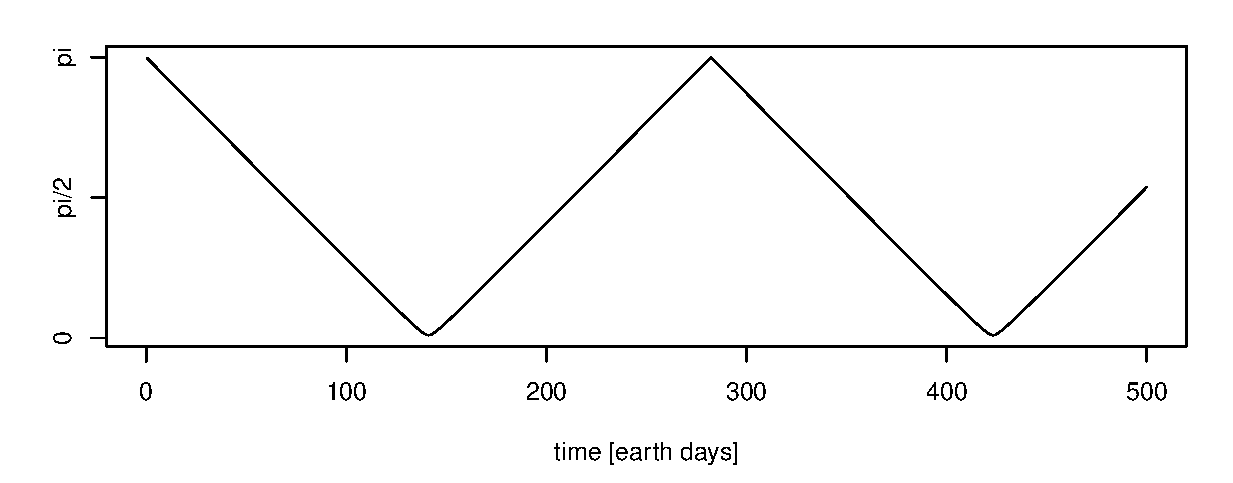
\includegraphics[width=\textwidth]{graphics/angle}
\caption{Absolute phase difference between the two moons.}
\label{fig:angle}
\end{figure}

\begin{figure}[h]
   \centering
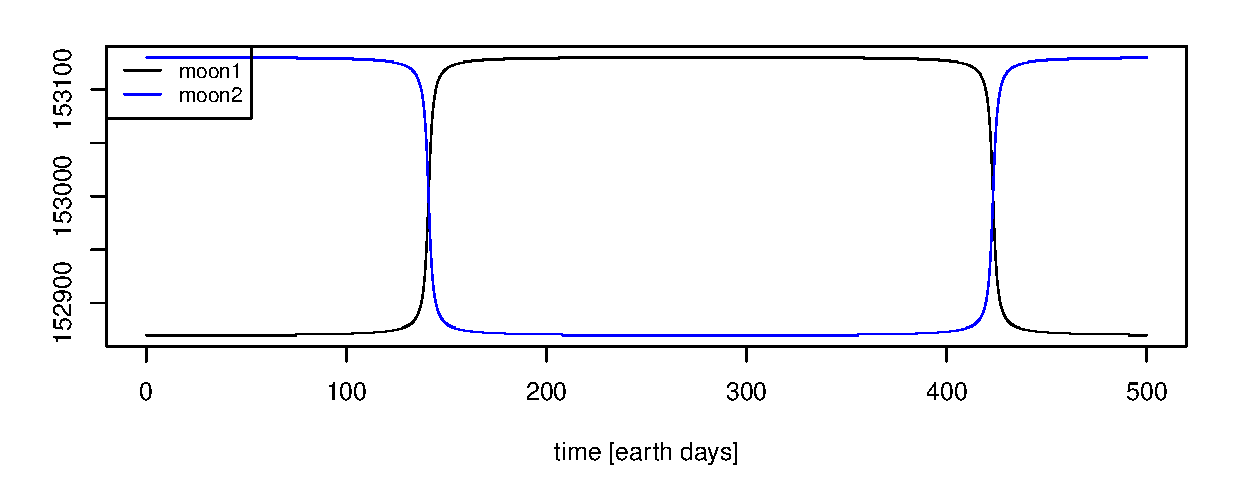
\includegraphics[width=\textwidth]{graphics/distance}
\caption{Distance from the moons to Saturn}
\label{fig:distance}
\end{figure}

The maximum error is predicted using the min step size and absolute error per step.
This is done by using the equation \ref{eq:NoSteps}.
Notations are borrowed from the NR library and book.

\begin{equation}
'Max.\ no.\ steps' = \frac{x_2 - x_1}{hmin}
\label{eq:NoSteps}
\end{equation}

$hmin$ was set to 0.1 km to avoid too many function-computations.
This gave a maximum number of steps to integrate the function of 5000.
From here, equation \ref{eq:accuracy} can be used to decide the highest accuracy needed to gain a maximum error of 10km.

\begin{equation}
accuracy = atoll *\ 'Max.\ no.\ steps'
\label{eq:accuracy}
\end{equation}

Using the numbers gained earlier the $atoll$, absolute error for one step, was decided to be $2\cdot10^{-3}$.

The actual maximum error in the current run is calculated with the StepperStoerm algorithm in NR.
Using that the actual number of iterations were 2931. The worst case error is 5.862 km.
Changing a few lines in the NR library gained, the error was output from the step function and passed on to the integrate function.
The single step error was then summed up and printed.
This gave an error of 1.50603 km. 

